\documentclass[english]{article}

\usepackage[latin9]{inputenc}
\usepackage[letterpaper]{geometry}
\geometry{verbose,tmargin=1in,bmargin=1in,lmargin=1in,rmargin=1in}
\usepackage{amsmath}
\usepackage{amssymb}
\usepackage{graphicx}

\newcommand{\grav}{\overrightarrow{g}}
\newcommand{\rotvec}{\overrightarrow{\theta}}

\title{ESE 650, Learning in Robotics, Spring 2016: Project4 \\
Yu-Cheng Lin}
\date{}

\begin{document}
\maketitle
\section*{Introduction}
In this project, we try to accomplish SLAM(simultaneous localization and mapping) based on the lidar scan of a humanoid robot. This problem is difficult because a map is required to recover the pose of a mobile robot, and the pose of the robot is required to construct the map. One approach to solve this problem is particle filter. This approach is better in most cases compared to a Kalman Filter. First, the particle filter can model any type of distribution instead of just gaussian. Secondly, as the number of landmarks grow, the number of states that the Kalman filter needs to keep track of grows as well. Since the inversion of matrix at the update step is $O(n^3)$, the Kalman Filter can become quite inefficient. The particle filter, although better than the Kalman filter for localization purposes, still has its weaknesses. As the odometry gets worse, the noise one must inject into the odomentry update. The more noise there is, the more particles are required to localize effectively. Also, the number of particle required at higher dimensions also grows rapidly. Lastly, the noise in all dimensions are not independent given a fixed number of particles. Since particle filter uses Monte Carlo sampling, if I choose to search a larger space in one dimension, I will get fewer samples in other dimensions too. This makes tuning difficult.
\section*{Implementation}
\subsection*{Grid-Based Particle Filter}
For a robot that uses Lidar as its perceptual sensor, a grid-based particle filter would work better than for example FastSLAM because all scans are indistinguishable. A grid-based approach has a predifined probability of $P(O|S)$, this is the distribution of the grid being occupied given that the scanner returns true. This distribution is used to update the map. For localization, the prediction step uses odometry with an injected gaussian noise. $P(x^{i}|odometry) = N(x^{i}, C)$, where the C stands for covariance. In this implementation, C is just a simple spherical covariance. Then, once prediction is complete, the correction step follows. The correction step aims to maximize the joint probability of $P(x|odometry)$ and $P(scan|x)$, which is proportional to the posterior $P(x|odometry, scan)$.\\
The particle filter uses a Monte Carlo method and importance sampling to model this distribution. $P(scan|x)$ is evaluated by the correlation of the existing local map and the hypothesis scans of each particle. The best particle is then picked and the weights are updated based on the posterior of each particle. Resampling is performed when a number of particles have weights so low that they are basically ineffective.
\subsection*{Hacks}
To improve the integrity of mapping, I figured that I can update the map only when I am sure the robot is localized properly. In this case, the correlation data can be used assuming that the scans between time steps vary slowly if we have the true pose of the robot. To accomplish this, I implemented a simple box filter on the moving average of the past 20 steps of correlation values, and the map is only updated when the new scan has at least, say 90 percent of the filtered value. This makes my mapping more stable, which improves localization as well.\\
In addition, at every update, I apply a sharpening kernel to the cells I am updating to discourage one-cell shifts of the map. The downside for this method is that I can clear out occupied cells if I have sparse readings, normally on the cells that are further away from the robot. The orders are map 0 through map3. 
\section*{Ground Detection}
In order to detect the ground, I incorporated the RGBD data into the SLAM. I first get a prior on the expected vector of the ground plane using the pitch of the head angle. Then, I projected the depth readings into point clouds in the camera frame given the depth camera calibration. Given the expected vector, I can do a selective RANSAC on the point cloud to find the best points on the ground plane. Lastly, the points are transformed into both the world frame and the RGB camera frame, and the pixel values in the RGB camera values are pasted onto the grid map in the world frame.\\
Interestingly, this method ends up picking up the ceiling on dataset 0 because the ground plane takes up way fewer points in the depth point cloud. This can be easily solved by constraining the y coordinates of the points in the camera frame. The results are quite interesting. 
\section*{Trainin Set Results}
\subsection*{Dead Reckoning}
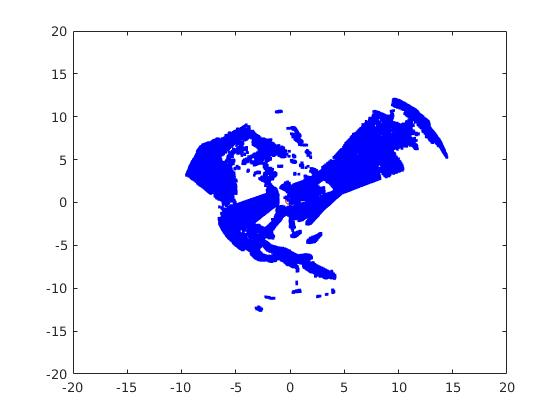
\includegraphics[scale=0.8]{map0dead.jpg}\\
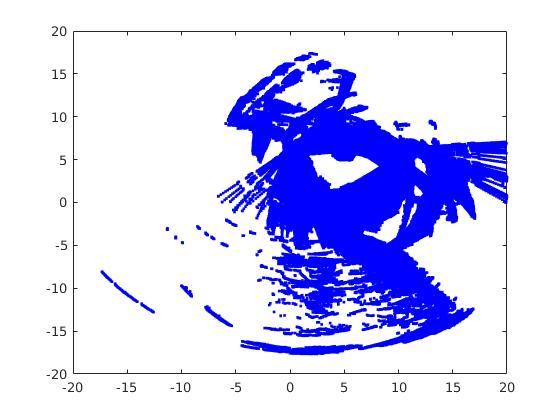
\includegraphics[scale=0.8]{map1dead.jpg}\\
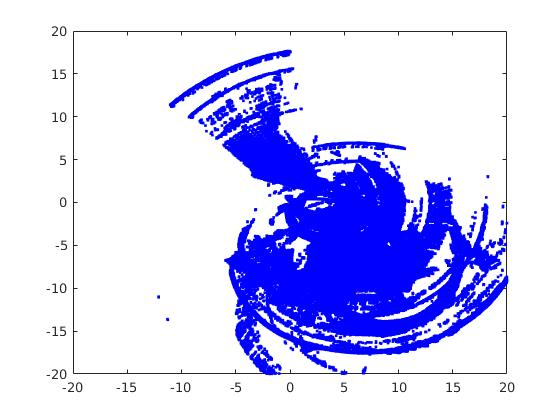
\includegraphics[scale=0.8]{map2dead.jpg}\\
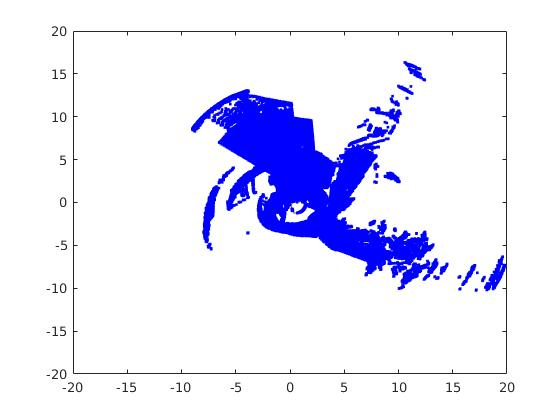
\includegraphics[scale=0.8]{map3dead.jpg}\\
\subsection*{SLAM}
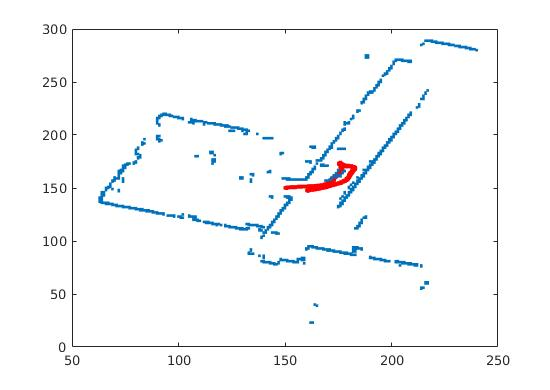
\includegraphics[scale=0.8]{map0.jpg}\\
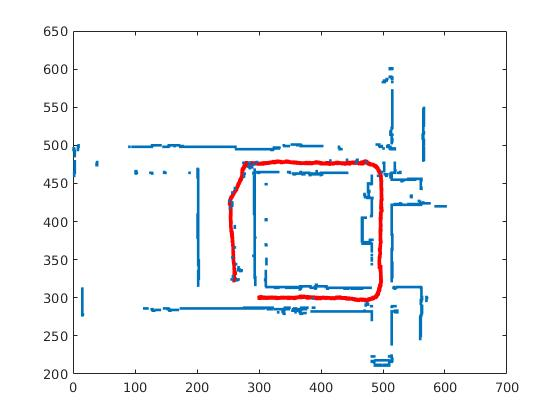
\includegraphics[scale=0.8]{map1.jpg}\\
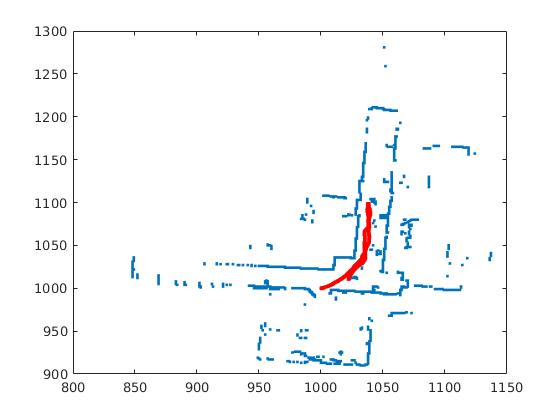
\includegraphics[scale=0.8]{map2.jpg}\\
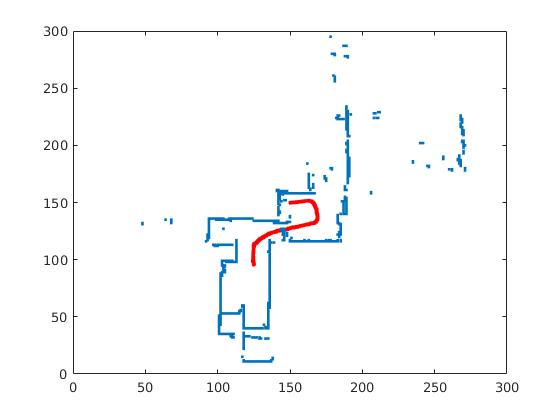
\includegraphics[scale=0.8]{map3.jpg}\\
\subsection*{Log Odds Map}
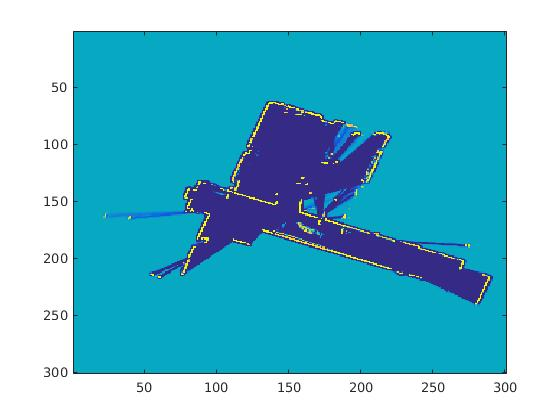
\includegraphics[scale=0.8]{logmap0.jpg}\\
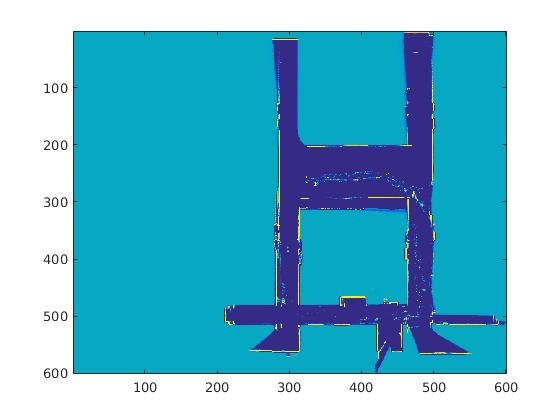
\includegraphics[scale=0.8]{logmap1.jpg}\\
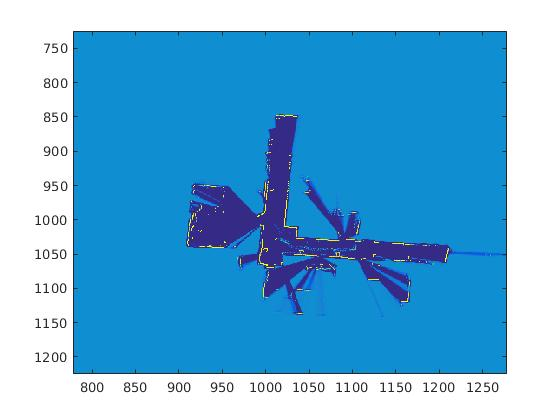
\includegraphics[scale=0.8]{logmap2.jpg}\\
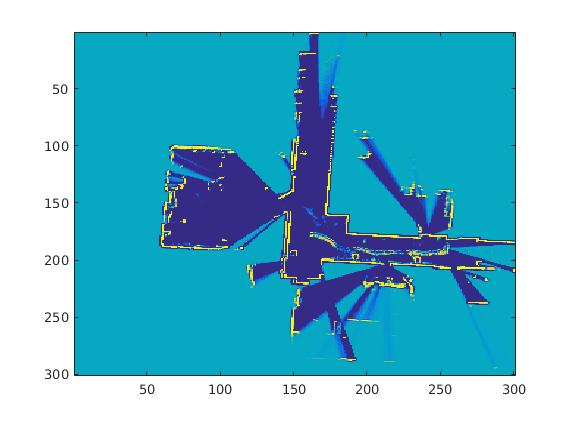
\includegraphics[scale=0.8]{logmap3.jpg}\\
\subsection*{Textured Map}
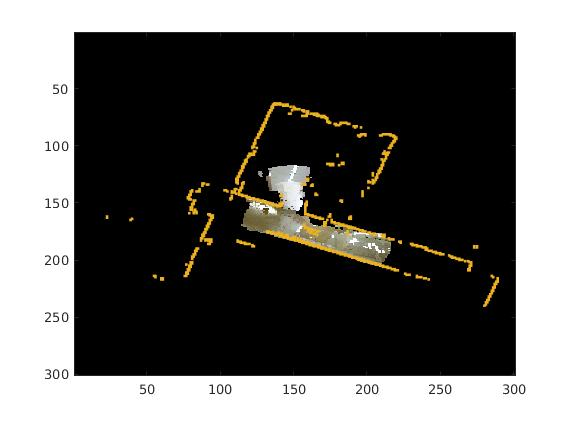
\includegraphics[scale=0.8]{map0texture.jpg}\\
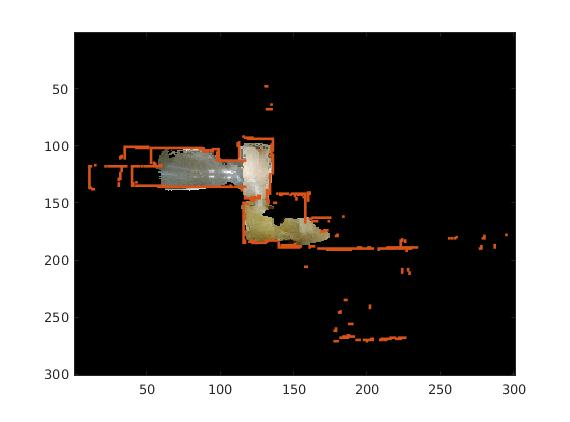
\includegraphics[scale=0.8]{map3texture.jpg}\\
\end{document}
